\documentclass{article}
\usepackage{lmodern}
\usepackage[charter]{mathdesign}
\usepackage[english]{babel}
\usepackage[utf8]{inputenc}

\usepackage{caption,subcaption}
\usepackage{fullpage}
\usepackage{color}
\usepackage{manfnt}
\usepackage{wasysym}
\usepackage{listings}
\usepackage{graphicx}
\usepackage{url}
%\usepackage{ulem}
\usepackage{marvosym}
%\usepackage{skull}
\usepackage{proof}
\usepackage{wrapfig}
\usepackage{array}

\title{{\bf Dynamic Scheduling in Halide}}
\author{Ben Blum \texttt{(bblum@andrew.cmu.edu)}}

\date{2013, December 16}

\newcommand\noob{\mathsf{noob}}
\newcommand\gibs{\mathsf{gibs}}
\newcommand\dps{\mathsf{dps}}
\newcommand\squig\rightsquigarrow
\newcommand\Coloneqq{\mathrel{\mathop{::}}=}
\newcommand\dmg{\text{\Laserbeam}}
\newcommand\delter\delta
\newcommand\alpher\alpha
\newcommand\defnor{\text{ }|\text{ }}

\newcommand\pimp{\mathop{\supset}}
\newcommand\pand{\mathop{\wedge}}
\newcommand\por{\mathop{\vee}}
\newcommand\ptrue{\top}
\newcommand\pfalse{\bot}


\begin{document}
\maketitle

\begin{figure}[h]
	\begin{center}
	\begin{tabular}{llllll}
		\begin{tabular}{l}
                \texttt{blur\_y(x,y) =} \\
                \texttt{~~~~(input(x, y-1) +}\\
                \texttt{~~~~~input(x, y~~) +}\\
                \texttt{~~~~~input(x, y+1))/3;}\\
                \\
                \texttt{blur\_x(x,y) =} \\
                \texttt{~~~~(blur\_y(x-1, y) +}\\
                \texttt{~~~~~blur\_y(x,~~~y) +}\\
                \texttt{~~~~~blur\_y(x+1, y))/3;}\\
		\end{tabular}
		& & & & &
		\begin{tabular}{l}
                \texttt{blur\_y\_far\_away(x,y) =} \\
                \texttt{~~~~(input(x, {\bf y-rand()}) +}\\
                \texttt{~~~~~input(x, y~~~~~~~) +}\\
                \texttt{~~~~~input(x, {\bf y+rand()}))/3;}\\
                \\
                \texttt{blur\_x\_far\_away(x,y) =} \\
                \texttt{~~~~(blur\_y({\bf x-rand()}, y) +}\\
                \texttt{~~~~~blur\_y(x,~~~~~~~~y) +}\\
                \texttt{~~~~~blur\_y({\bf x+rand()}, y))/3;}\\
		\end{tabular}

	\end{tabular}
	\end{center}
	\caption{Static and dynamic data dependencies in Halide. On the left, a 3x3 blur (the canonical example Halide program) need only reference input data up to 1 pixel away in each direction for each output pixel. On the right, the algorithm is modified such that the compiler cannot statically know which input pixels each output pixel may reference.}
	\label{fig:intro}
\end{figure}

%%%%%%%%%%%%%%%%%%%%%%%%%%%%%%%%%%%%%%%%%%%%%%%%%%%%%%%%%%%%%%%%%%%%%%%%%%%%%%%%
\section{Introduction}

Halide~\cite{halide} is a programming language for image processing pipelines designed to separate the concerns of performance and expressivity. The programming model is functional, representing images as functions from pixel coordinates to colour values, and representing each pass of an image processing algorithm as a function from images to images. Once implemented, the programmer's algorithm is then automatically parallelized by the Halide runtime, taking into account considerations such as how to split each pass into parallel tiles and the data dependencies between two consecutive passes.
The structure of the generated loop nest and the function calls therein is known as the {\em function schedule}.

One weakness of Halide is its inability to express image processing passes that don't operate uniformly across their domain; i.e., algorithms whose data dependencies on portions of previous passes cannot be known statically.
Figure~\ref{fig:intro} above contrasts two simple example algorithms, showcasing the difference between static and dynamic data dependencies.

In this project I investigate and implement {\em dynamic function scheduling}, a new language feature for Halide to support such algorithms.
My approach allows the computations for early pipeline stages to be cached across loop iterations of later stages, so that the results may be reused when data dependencies happen to coincide on the same location, saving redundant computation of a possibly expensive intermediate function.
The principal contribution of this work is the implementation and performance evaluation of {\em dynamic scheduling at pixel granularity}. I also investigated dynamic scheduling at coarser (e.g. tile) granularities, with which entire loop iterations may be skipped. However, the problem was more difficult than anticipated, so I instead provide some discussion and a design sketch for future work.

%%%%%%%%%%%%%%%%%%%%%%%%%%%%%%%%%%%%%%%%%%%%%%%%%%%%%%%%%%%%%%%%%%%%%%%%%%%%%%%%
\section{Motivation}

\definecolor{grey}{RGB}{127,127,127}
\definecolor{darkcyan}{RGB}{0,127,127}
\definecolor{olivegreen}{RGB}{0,127,0}
\definecolor{violet}{RGB}{127,0,127}
\definecolor{brickred}{RGB}{127,0,0}
\definecolor{brown}{RGB}{127,63,0}
\definecolor{orange}{RGB}{192,96,0}
\newcommand\hilight[2]{\color{#1}#2\color{black}}


\begin{figure}[t]
	\begin{center}
	\begin{subfigure}[b]{0.45\textwidth}
		\begin{center}
		\begin{tabular}{l}
		{\em User-provided schedule:} \\
		\\
		\hilight{blue}{\texttt{blur\_x /* nothing special */;}} \\
		\hilight{olivegreen}{\texttt{blur\_y.store\_root().compute\_root();}} \\
		\\
		{\em Compiler-generated code:} \\
		\\
                \texttt{\hilight{olivegreen}{float~blur\_y[HEIGHT][WIDTH];}} \\
                \texttt{\hilight{olivegreen}{for~(row~=~0~to~HEIGHT)~\{}} \\
                \texttt{\hilight{olivegreen}{~~for~(col~=~0~to~WIDTH)~\{}} \\
                \texttt{\hilight{olivegreen}{~~~~blur\_y[row][col] = ...;}}\\
                \texttt{\hilight{olivegreen}{~~\}}} \\
                \texttt{\hilight{olivegreen}{\}}} \\
		\\
                \texttt{\hilight{blue}{float~blur\_x[HEIGHT][WIDTH];}} \\
                \texttt{\hilight{blue}{for~(row~=~0~to~HEIGHT)~\{}} \\
                \texttt{\hilight{blue}{~~for~(col~=~0~to~WIDTH)~\{}} \\
                \texttt{\hilight{blue}{~~~~blur\_x[row][col] = ...;}}\\
                \texttt{\hilight{blue}{~~\}}} \\
                \texttt{\hilight{blue}{\}}} \\
		\end{tabular}
		\end{center}
		\caption{\texttt{blur\_x} and \texttt{blur\_y} are scheduled separately. This schedule, while easy to understand, offers poor locality (values computed are not used until a full image traversal later) and poor parallelism (creating one thread per row or column of pixels both floods the system with too many threads and creates cache contention).}
		\label{fig:scheds-a}
	\end{subfigure}
	\qquad
	\begin{subfigure}[b]{0.5\textwidth}
		\begin{center}
		\begin{tabular}{l}
		{\em User-provided schedule:} \\
		\\
                \hilight{blue}{\texttt{blur\_x.tile(x, y, x2, y2, 8, 8).parallel(y);}}\\
                \hilight{olivegreen}{\texttt{blur\_y.store\_at(blur\_x, x).compute\_at(blur\_x, y2);}}\\
                \\
		{\em Compiler-generated code:} \\
		\\
                \texttt{\hilight{blue}{float~blur\_x[HEIGHT][WIDTH];}} \\
                \texttt{\hilight{blue}{PARALLEL for~(row~=~0~to~8)~\{}} \\
                \texttt{\hilight{blue}{~~for~(col~=~0~to~8)~\{}} \\
                \texttt{\hilight{olivegreen}{~~~~float~blur\_y[HEIGHT/8 + 2][WIDTH/8 + 2];}} \\
                \texttt{\hilight{blue}{~~~~for~(row2~=~0~to~WIDTH/8 + 2)~\{}} \\
                \texttt{\hilight{olivegreen}{~~~~~~for~(col2~=~0~to~WIDTH/8 + 2)~\{}} \\
                \texttt{\hilight{olivegreen}{~~~~~~~~blur\_y[row2][col2]~=~...;}} \\
                \texttt{\hilight{olivegreen}{~~~~~~\}}} \\
                \texttt{\hilight{blue}{~~~~~~for~(col2~=~0~to~WIDTH/8)~\{}} \\
                \texttt{\hilight{blue}{~~~~~~~~blur\_x[row*8~+~row2][col*8~+~col2]~=~...;}} \\
                \texttt{\hilight{blue}{~~~~~~\}}} \\
                \texttt{\hilight{blue}{~~~~\}}} \\
                \texttt{\hilight{blue}{~~\}}} \\
                \texttt{\hilight{blue}{\}}} \\
		\end{tabular}
		\end{center}
		\caption{\texttt{blur\_x} is tiled in 8-fold splits in each dimension, and \texttt{blur\_y} is scheduled at the tile level within \texttt{blur\_x}. This schedule offers good locality (values are used soon after being computed) and good parallelism (one thread per tile; tile size can be customized).}
		\label{fig:scheds-b}
	\end{subfigure}
	\end{center}
	\caption{Two example function schedules for the two-stage blur algorithm shown in Figure~\ref{fig:intro}.}
	\label{fig:scheds}
\end{figure}

The high concept of Halide is to separate the logic of an image processing algorithm from the order in which the functions for each stage are scheduled. Figure~\ref{fig:scheds} shows two possible schedules for my example algorithm, and discusses the performance characteristics of each.
Though Figure~\ref{fig:scheds-b} is more cache-friendly and offers superior paralellism opportunity, a notable disadvantage is that some computation is duplicated across tiles. This is shown in the extra 2 pixels computed for \texttt{blur\_y} in each dimension. In this example, the overhead is minor, as Halide can statically reason about the maximum extra ``padding'' that \texttt{blur\_y} must compute for each tile of \texttt{blur\_x}.

However, this extra computation can become a significant problem when the dependencies between the algorithm's stages are computed at runtime and hence are not available for compile-time reasoning, as in the PatchMatch algorithm~\cite{patchmatch} and in edge detection. If the user wishes to use a cache-friendly, highly-parallel function schedule, as in Figure~\ref{fig:scheds-b}, Halide must make a conservative estimate regarding how much extra padding is required, resulting in extra work duplication.

To get a sense for how much extra unnecessary computation can arise, I introduce a sample two-stage Halide program in which the second stage (\texttt{flip()}) dynamically computes which pixels it requires from the first stage (\texttt{invert()}). This program is described in Figures~\ref{fig:flip} and~\ref{fig:flip-code}. I then ran this program on a test image using the simple schedule from Figure~\ref{fig:scheds-a} and using several nested schedules as in Figure~\ref{fig:scheds-b}. I found that in the former situation, 13,068 calls to \texttt{invert()} were required, while in the latter, \texttt{invert()} was invoked anywhere between 252,648 to 7,847,400 times depending on the schedule used.
Hence, the motivation for {\em dynamic scheduling} is to extend Halide's ability to avoid duplicate work to apply to this wider range of algorithms.

\begin{figure}[t]
	\begin{tabular}{cc}
	\begin{subfigure}[b]{0.45\textwidth}
		\begin{center}
		\includegraphics[width=0.85\textwidth]{canoe-0.png}
		\end{center}
		\caption{Original input image.}
	\end{subfigure} &
	\begin{subfigure}[b]{0.45\textwidth}
		\begin{center}
		\includegraphics[width=0.85\textwidth]{canoe-1.png}
		\end{center}
		\caption{Stage 1 is a simple value-invert of each input pixel.}
		\label{fig:invert}
	\end{subfigure} \\
	& \\
	\begin{subfigure}[b]{0.45\textwidth}
		\begin{center}
		\includegraphics[width=0.85\textwidth]{canoe-2.png}
		\end{center}
		\caption{The core of stage 2 is a transformation across a vector field, which maps points near the center to the corners and points near the corners to the center, followed by a 3x3 blur. The blur causes each output pixel to depend on multiple input pixels, which allows for the possibility of work duplication.}
		\label{fig:flip-blur-1}
	\end{subfigure} &
	\begin{subfigure}[b]{0.45\textwidth}
		\begin{center}
		\includegraphics[width=0.85\textwidth]{canoe-3.png}
		\end{center}
		\caption{Final output. Stage 2 is altered to only apply the vector field to pixels when their colour value is darker than a certain threshold. This condition, which depends on a nondeterministic property of the input image, prevents Halide's optimizations from reasoning about the data dependencies between the two stages.}
		\label{fig:flip-blur-2}
	\end{subfigure}
	\end{tabular}
	\caption{Our sample image processing program consists of two stages, \texttt{invert()} (shown in \ref{fig:invert}) and \texttt{flip()} (shown in \ref{fig:flip-blur-1} and \ref{fig:flip-blur-2}). I designed this program expressly to create dynamic data dependencies with wide ranges across the image, to ensure a static function schedule could not avoid duplicating work.}

	\label{fig:flip}
\end{figure}

\begin{figure}[t]
	\begin{center}
	\begin{tabular}{l}
\texttt{\hilight{olivegreen}{Var}~x(\hilight{brickred}{"column"}), y(\hilight{brickred}{"row"}), c(\hilight{brickred}{"colour"});} \\
\\
\texttt{\hilight{darkcyan}{/* Stage 1 */}} \\
\texttt{\hilight{olivegreen}{Func}~invert(\hilight{olivegreen}{Func}~input)~\{} \\
\texttt{~~~~\hilight{olivegreen}{Func}~f(\hilight{brickred}{"invert"});} \\
\texttt{~~~~f(x,~y,~c)~=~\hilight{brickred}{1}~-~input(x,~y,~c);~} \\
\texttt{~~~~\hilight{brown}{return}~f;} \\
\texttt{\}} \\
\\
\texttt{\hilight{darkcyan}{/* The vector field used in stage 2 */}} \\
\texttt{\#define~vf\_x(image,~do\_flip,~x)~(\hilight{brown}{select}(do\_flip,~x,~((\hilight{brickred}{3}~*~image.width()~~/~\hilight{brickred}{2})~-~x)))} \\
\texttt{\#define~vf\_y(image,~do\_flip,~y)~(\hilight{brown}{select}(do\_flip,~y,~((\hilight{brickred}{3}~*~image.height()~/~\hilight{brickred}{2})~-~y)))} \\
\texttt{} \\
\texttt{\hilight{darkcyan}{/* Stage 2 */}} \\
\texttt{\hilight{olivegreen}{Func}~flip(\hilight{olivegreen}{Image}<\hilight{olivegreen}{float}>~\&i,~\hilight{olivegreen}{Func}~input)~\{} \\
\texttt{~~~~\hilight{olivegreen}{Expr}~do\_flip~=~input(x,~y,~c)~>~\hilight{brickred}{0.5f};} \\
\texttt{~~~~\hilight{olivegreen}{Func}~f(\hilight{brickred}{"flip"});} \\
\texttt{~~~~f(x,~y,~c)~=} \\
\texttt{~~~~~~~~(input(vf\_x(i,~do\_flip,~x-\hilight{brickred}{1}),~vf\_y(i,~do\_flip,~y-\hilight{brickred}{1}),~c)~+} \\
\texttt{~~~~~~~~~\hilight{darkcyan}{/* ... intermediate coordinates of 3x3 blur omitted ... */}} \\
\texttt{~~~~~~~~~input(vf\_x(i,~do\_flip,~x+\hilight{brickred}{1}),~vf\_y(i,~do\_flip,~y+\hilight{brickred}{1}),~c))~/~\hilight{brickred}{9};} \\
\texttt{~~~~\hilight{brown}{return}~f;} \\
\texttt{\}} \\

	\end{tabular}
	\end{center}
	\caption{Selected code from the implementation of the sample image processing program.}
	\label{fig:flip-code}
\end{figure}

%%%%%%%%%%%%%%%%%%%%%%%%%%%%%%%%%%%%%%%%%%%%%%%%%%%%%%%%%%%%%%%%%%%%%%%%%%%%%%%%
\section{Design and Implementation}

% This section discusses how I organized my code to implement this project. The reader seeking a research perspective will likely be disinterested, while the reader seeking to extend or maintain my work may well find this the most useful section in the report.

\subsection{Overview}

Conceptually, my goal for dynamic function scheduling as a Halide language feature was as follows. In addition to the existing directives \texttt{compute\_at()}, \texttt{store\_at()}, and so on which users may call on their \texttt{Func} objects, supplying appropriate loop variable arguments, I would add a new directive \texttt{compute\_lazy()}.

{\bf Pixel-granularity dynamic scheduling.} Used with no arguments, this directive would instruct Halide to allocate a ``bitmask'', an array of booleans with the same dimensions as the array used to store the function's results themselves. Halide would then surround any expression which computed a value to store in the array at a certain index with a check to this bitmask at the same index, which would cause the expression to be bypassed if a value for that index had been computed before. I refer to this as dynamic scheduling at {\em pixel granularity} because there is one bitmask check per expression that would compute a value for a single pixel. In Figure~\ref{fig:dynamic-pixel} I show sample code that Halide would generate for a program that used pixel-level dynamic scheduling.

{\bf Tile-granularity dynamic scheduling.} If the user supplies a loop variable as the argument to \texttt{compute\_lazy()}, Halide will place the conditional check just inside the loop corresponding to that variable, instead of immediately around the store operation inside the innermost loop. This results in caching of already-computed tiles (or rows or columns as the case may be). This can provide several benefits: performing the conditional check only once per group of pixels saves the overhead of a branch, allows vectorizing the innermost loops, and allows skipping entire iterations across loop ranges in addition to just skipping a function call. In Figure~\ref{fig:dynamic-tile} I show sample code that Halide would generate for a program that used tile-level dynamic scheduling.

\subsection{Code Generation}

Inside the compiler, the dynamic schedule configuration is stored in a \texttt{Func}'s \texttt{Schedule} object as a \texttt{LoopLevel} named \texttt{lazy\_level}, alongside the existing configurations \texttt{store\_level} and \texttt{compute\_level}. Unlike the latter two, however, the \texttt{lazy\_level} is not defined in terms of the loop variable of a different function, but rather for one of the function's own loop variables. Hence, \texttt{lazy\_level.func} always refers to the containing function.

The code generation itself occurs during the \texttt{Lower} phase of compilation, between the \texttt{schedule\_functions()} phase (found in \texttt{Lower.cpp}) and the \texttt{storage\_flattening()} phase (found in \texttt{StorageFlattening.cpp}). The former processes the \texttt{lazy\_level} configuration and generates IR to represent it, and the latter converts those IR nodes into conventional IR that can be code-generated. For this purpose I added a new type of IR node, \texttt{DynamicStmt} (found in \texttt{IR.h}), which represents the ``if not-in-cache then compute; mark-cache; end'' pattern.

\begin{itemize}
	\item {\bf Function Scheduling.} This phase converts the dynamic schedule configuration into IR in two places. The first is when it generates a \texttt{Realize} node (in \texttt{build\_realize()}); it simply sets the node's \texttt{lazy} flag to \texttt{true} if the associated function's \texttt{lazy\_level} was set.\footnote{
	I experimented here with computing and storing an expression representing the necessary size for the bitmask, rather than just a boolean. Future work may find this approach worth doing after all.}
	The second is when building a function's loop nest (in \texttt{build\_provide\_loop\_nest()}); when the approprate loop level is encountered, it inserts a \texttt{DynamicStmt} node between the \texttt{For} loop and its body.
	\item {\bf Storage Flattening.} This phase visits the IR described above and ``flattens'' it into arrays more reminiscent of the C memory model. In \texttt{visit(Realize *)}, where it makes the \texttt{Allocate} node for the function's computed results, it now also will make another \texttt{Allocate} and a brief initialization loop if \texttt{realize->lazy} is set. Second, in \texttt{visit(DynamicStmt *)}, it converts the \texttt{DynamicStmt} node into a conventional \texttt{IfThenElse} node using the provided index for the allocated bitmask.
\end{itemize}

\subsection{Legality Checking}

During the function scheduling in \texttt{Lower.cpp} Halide must also check that a specified dynamic schedule is legal. I currently check for the following cases:

\begin{itemize}
	\item {\bf Vectorized loop.} If any of the loops between the \texttt{store\_level} and the \texttt{lazy\_level} are vectorized, it may not make sense to emit a check which conditionally skips much of the computation. Though it would make sense to generate code for a single boolean check around a single pixel computation, with more sophisticated tile-level dynamic scheduling the vectorized execution might behave pathologically (especially if the conditional check involves traversing a sophisticated data structure as suggested in Section~\ref{sec:future}).
	\item {\bf Parallel loop.} If any of the loops between the \texttt{store\_level} and the \texttt{lazy\_level} are parallelized, then one thread attempting to record the result of a computation might race with another thread attempting to use that result. With x86's sequentially-consistent memory model and the simple boolean check, this is not an issue, but when compiling for ARM or using a more sophisticated data structure for memoizing Halide would need to emit memory barriers at best and locks at worst. This is not infeasible to implement, but raises research questions of its own and so is left to future work.
	\item {\bf Update phase.} Dynamic scheduling is not (yet) compatible with functions which have an update phase in their \texttt{Pipeline} node, which can arise when the user provides a reduction definition. This is merely a case I did not consider in detail, and may well be possible to handle.
\end{itemize}

\subsection{Problems with Tile-Level Dynamic Scheduling}
\label{sec:problem}

\begin{wrapfigure}{r}{0.28\textwidth}
	\begin{center}
	\includegraphics[width=0.2\textwidth]{bloopers/01.png}
	\end{center}
	\caption{Dynamic scheduling at tile granularity can fail to compute results for some pixels, using uninitialized values instead. (Compare to the expected output in Figure~\ref{fig:correct-output}.)}
	\label{fig:uh-oh}
\end{wrapfigure}

To cache computed results at coarser-than-pixel granularity, I used the coordinate of the ``top left'' pixel within the block as the index into the bitmask. Unfortunately, this proved inadequate in some cases, leading to the program erroneously believing it had aleady computed a block of pixels and using uninitialized values for some pixels.

In Figure~\ref{fig:dynamic-tile}, note the two lines of code marked \texttt{XXX}. These lines compute the bounds of the \texttt{col\_i} dimension, and their values depend on the value of the outer \texttt{col} loop variable, which varies across iterations. Hence, on one iteration we might compute \texttt{invert} values for the range (0,0) to (0,14), store that we had already computed the row starting at (0,0), then later skip computing values for the range (0,0) to (0,15), leaving the last pixel undefined. This behaviour is shown in Figure~\ref{fig:uh-oh}, where the rightmost column of the image has been generated with undefined values.

Note that this problem only arises with some schedules; for example, changing \texttt{invert.store\_at(flip, row);} to \texttt{store\_at(flip, col);} would prevent tiles of different sizes from arising. Nevertheless, a correct implementation in the general case must memoize the dimensions of each tile computed in addition to the location. Section~\ref{sec:future} discusses potential solutions.

\subsection{Code}

The reader should feel free to find and peruse my code at \texttt{https://github.com/bblum/Halide}. During the weeks following this submission I will polish it and submit a pull request upstream.

\pagebreak
\begin{figure}[h!]
	\begin{center}
	\begin{subfigure}[b]{0.475\textwidth}
		\begin{center}
		\begin{tabular}{l}
		{\em User-provided schedule:} \\
		\\
                \hilight{blue}{\texttt{flip.tile(col, row, col2, row2, 8, 8);}} \\
                \hilight{olivegreen}{\texttt{invert.store\_at(flip, row);}} \\
		\hilight{olivegreen}{\texttt{invert.compute\_at(invert, row2);}}\\
                {\bf \hilight{orange}{\texttt{invert.compute\_lazy();}}} \\
                \\
		{\em Compiler-generated code:} \\
		\\
                \texttt{\hilight{blue}{float~flip[HEIGHT][WIDTH];}} \\
                \texttt{\hilight{blue}{for~(row~=~0~to~8)~\{}} \\
                \texttt{\hilight{olivegreen}{~~float~invert[...][...];}} \\
		{\bf \texttt{\hilight{orange}{~~bool~result\_computed[...][...];}}} \\
                \texttt{\hilight{blue}{~~for~(col~=~0~to~8)~\{}} \\
                \texttt{\hilight{blue}{~~~~for~(row2~=~0~to~WIDTH/8)~\{}} \\
                \texttt{\hilight{olivegreen}{~~~~~~let min\_row = ...;}} \\
                \texttt{\hilight{olivegreen}{~~~~~~let max\_row = ...;}} \\
                \texttt{\hilight{olivegreen}{~~~~~~let min\_col = ...;}} \\
                \texttt{\hilight{olivegreen}{~~~~~~let max\_col = ...;}} \\
                \texttt{\hilight{olivegreen}{~~~~~~for~(row\_i~=~min\_row~to~max\_row)~\{}} \\
                \texttt{\hilight{olivegreen}{~~~~~~~~for~(col\_i~=~min\_col~to~max\_col)~\{}} \\
		{\bf \texttt{\hilight{orange}{~~~~~~~~~~if (!result\_computed[...][...]) \{}}} \\
                \texttt{\hilight{olivegreen}{~~~~~~~~~~~~invert[row\_i][col\_i]~=~...;}} \\
		{\bf \texttt{\hilight{orange}{~~~~~~~~~~~~result\_computed[...][...]~=~TRUE;}}} \\
		{\bf \texttt{\hilight{orange}{~~~~~~~~~~\}}}} \\
                \texttt{\hilight{olivegreen}{~~~~~~~~\}}} \\
                \texttt{\hilight{olivegreen}{~~~~~~\}}} \\
                \texttt{\hilight{blue}{~~~~~~for~(col2~=~0~to~WIDTH/8)~\{}} \\
                \texttt{\hilight{blue}{~~~~~~~~flip[...][...]~=~...;}} \\
                \texttt{\hilight{blue}{~~~~~~\}}} \\
                \texttt{\hilight{blue}{~~~~\}}} \\
                \texttt{\hilight{blue}{~~\}}} \\
                \texttt{\hilight{blue}{\}}} \\
		\end{tabular}
		\end{center}
		\caption{Dynamic scheduling at pixel granularity. The directive \texttt{invert.compute\_lazy()} with no arguments is shorthand for supplying \texttt{invert}'s innermost loop variable (in this case, \texttt{col\_i}).}
		\label{fig:dynamic-pixel}
	\end{subfigure}
	\qquad
	\begin{subfigure}[b]{0.475\textwidth}
		\begin{center}
		\begin{tabular}{l}
		{\em User-provided schedule:} \\
		\\
                \hilight{blue}{\texttt{flip.tile(col, row, col2, row2, 8, 8);}} \\
                \hilight{olivegreen}{\texttt{invert.store\_at(flip, row);}} \\
		\hilight{olivegreen}{\texttt{invert.compute\_at(invert, row2);}}\\
                {\bf \hilight{orange}{\texttt{invert.compute\_lazy(row\_i);}}} \\
                \\
		{\em Compiler-generated code:} \\
		\\
                \texttt{\hilight{blue}{float~flip[HEIGHT][WIDTH];}} \\
                \texttt{\hilight{blue}{for~(row~=~0~to~8)~\{}} \\
                \texttt{\hilight{olivegreen}{~~float~invert[...][...];}} \\
		{\bf \texttt{\hilight{orange}{~~bool~result\_computed[...][...];}}} \\
                \texttt{\hilight{blue}{~~for~(col~=~0~to~8)~\{}} \\
                \texttt{\hilight{blue}{~~~~for~(row2~=~0~to~WIDTH/8)~\{}} \\
                \texttt{\hilight{olivegreen}{~~~~~~let min\_row = ...;}} \\
                \texttt{\hilight{olivegreen}{~~~~~~let max\_row = ...;}} \\
                \texttt{\hilight{olivegreen}{~~~~~~let min\_col = ...; // XXX}} \\
                \texttt{\hilight{olivegreen}{~~~~~~let max\_col = ...; // XXX}} \\
                \texttt{\hilight{olivegreen}{~~~~~~for~(row\_i~=~min\_row~to~max\_row)~\{}} \\
		{\bf \texttt{\hilight{orange}{~~~~~~~~if (!result\_computed[...][...]) \{}}} \\
                \texttt{\hilight{olivegreen}{~~~~~~~~~~for~(col\_i~=~min\_col~to~max\_col)~\{}} \\
                \texttt{\hilight{olivegreen}{~~~~~~~~~~~~invert[row\_i][col\_i]~=~...;}} \\
                \texttt{\hilight{olivegreen}{~~~~~~~~~~\}}} \\
		{\bf \texttt{\hilight{orange}{~~~~~~~~~~result\_computed[...][...]~=~TRUE;}}} \\
		{\bf \texttt{\hilight{orange}{~~~~~~~~\}}}} \\
                \texttt{\hilight{olivegreen}{~~~~~~\}}} \\
                \texttt{\hilight{blue}{~~~~~~for~(col2~=~0~to~WIDTH/8)~\{}} \\
		\texttt{\hilight{blue}{~~~~~~~~flip[...][...]~=~...;}} \\
                \texttt{\hilight{blue}{~~~~~~\}}} \\
                \texttt{\hilight{blue}{~~~~\}}} \\
                \texttt{\hilight{blue}{~~\}}} \\
                \texttt{\hilight{blue}{\}}} \\
		\end{tabular}
		\end{center}
		\caption{Dynamic scheduling at tile granularity. Here, the ``tile'' is simply the row denited by the variable \texttt{row\_i}. Simply using a single boolean for each tile can be unsound in some cases, as discussed in Section~\ref{sec:problem}.}
		\label{fig:dynamic-tile}
	\end{subfigure}
	\end{center}
	\caption{Generated code listings for dynamic function schedules, at both pixel and tile granularity. In addition to highlighting the code associated with the \hilight{blue}{flip}~and \hilight{olivegreen}{invert}~stages of the algorithm, I also {\bf \hilight{orange}{emphasize}} the additional code generated for dynamic scheduling.}
	\label{fig:dynamic}
\end{figure}

\pagebreak

%%%%%%%%%%%%%%%%%%%%%%%%%%%%%%%%%%%%%%%%%%%%%%%%%%%%%%%%%%%%%%%%%%%%%%%%%%%%%%%%
\section{Evaluation}

To evaluate dynamic scheduling I sought to answer the following questions.

\begin{itemize}
	\item How much duplicate work does dynamic scheduling let us avoid?
	\item How does the amount of duplicate work avoided and the execution time vary when different function schedules are used?
\end{itemize}

To approach these questions I ran experiments with input images of three different sizes using 8 different function schedules. I list the schedules used in Figure~\ref{fig:eval-scheds}, and show the images in Figure~\ref{fig:eval-images}.

\begin{figure}[h]
	\begin{center}
	\begin{tabular}{c|c}
		x-axis label & schedule used for \texttt{invert()} \\
		\hline
                1 & \texttt{invert.store\_at(flip, c).compute\_at(flip, yi);~} \\
                2 & \texttt{invert.store\_at(flip, c).compute\_at(flip, xi);~} \\
                3 & \texttt{invert.store\_at(flip, y).compute\_at(flip, x);~~} \\
                4 & \texttt{invert.store\_at(flip, y).compute\_at(flip, yi);~} \\
                5 & \texttt{invert.store\_at(flip, y).compute\_at(flip, xi);~} \\
                6 & \texttt{invert.store\_at(flip, x).compute\_at(flip, yi);~} \\
                7 & \texttt{invert.store\_at(flip, x).compute\_at(flip, xi);~} \\
                8 & \texttt{invert.store\_at(flip, yi).compute\_at(flip, xi);} 
	\end{tabular}
	\end{center}
	\caption{All experiments used the schedule \texttt{flipped.tile(x, y, xi, yi, 2, 2);}. On the subsequent graphs in this evaluation, the x-axis labels correspond to the corresponding schedule for \texttt{invert} here.}
	\label{fig:eval-scheds}
\end{figure}
\begin{figure}[h]
        \begin{center}
        \begin{tabular}{ccc}
	\begin{subfigure}[b]{0.22\textwidth}
        \includegraphics[width=\textwidth]{gradient.png} \\
        \\
        \includegraphics[width=\textwidth]{gradient-output.png} \\
        \caption{Small image (64x64)}
        \label{fig:correct-output}
	\end{subfigure}
	&
	\begin{subfigure}[b]{0.34\textwidth}
        \includegraphics[width=\textwidth]{readers-writers.png} \\
        \\
        \includegraphics[width=\textwidth]{rw-output.png} \\
        \caption{Medium image (400x261)}
	\end{subfigure}
	&
	\begin{subfigure}[b]{0.335\textwidth}
        \includegraphics[width=\textwidth]{canoe-0.png} \\
        \\
        \includegraphics[width=\textwidth]{canoe-3.png} \\
        \caption{Large image (963x642)}
	\end{subfigure}
        \end{tabular}
        \caption{Images used for evaluation (top), and the outputs given by the invert/flip algorithm (bottom).}
        \label{fig:eval-images}
        \end{center}
\end{figure}

\begin{figure}[h]
	\begin{center}
	\includegraphics[width=0.47\textwidth]{graphs/small.pdf}
	\end{center}
	\caption{Analysis of how much duplicate work was saved for the small image. Lower is better.}
	\label{fig:graph-trace}
\end{figure}
\begin{figure}[h]
	\begin{center}
	\includegraphics[width=0.47\textwidth]{graphs/medium.pdf} \quad
	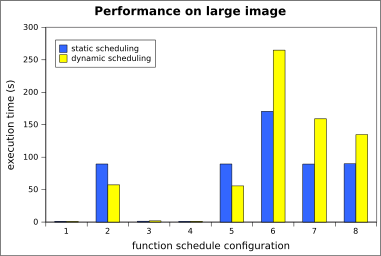
\includegraphics[width=0.47\textwidth]{graphs/large.pdf}
	\end{center}
	\caption{Performance results for the medium and large images. Lower is better.}
	\label{fig:graph-perf}
\end{figure}

\subsection{Work Saved}

For the small input image, I used Halide's tracing facility to measure the number of pixels computed by the \texttt{invert()} operation (\texttt{invert.trace\_stores()}), comparing the numbers obtained from dynamic and from static scheduling. For each schedule, the difference in this number represents the amount of computation saved.

Figure~\ref{fig:graph-trace} shows this experiment's results. We can see that in some cases, several orders of magnitude of work are saved; in some, a modest amount of work is saved; and in some it makes no difference. Naturally dynamic scheduling never creates additional \texttt{invert()} calls.

\subsection{Peformance Discussion}

For the medium and large input image I measured the elapsed wall clock time during execution, running both statically and dynamically. Figure~\ref{fig:graph-perf} shows this experiment's results. The performance patterns are similar between the medium and large images, apart from the obvious difference in number of total seconds taken.

One notable anomaly is that in schedules 6, 7, and 8, performance is actually worse with dynamic scheduling than with static scheduling. I attribute this to the fact that in these schedules the \texttt{invert()} code is confined to the innermost loop levels of \texttt{flip()}, which causes \texttt{invert()}'s buffer to be freed and re-allocated many times, thereby hurting the potential for saving computation across loop iterations.
Though these schedules still reduce the number of \texttt{invert()} calls (as shown in the previous experiment), they fail to compensate for the incidental overhead of using dynamic scheduling to begin with -- that is, the cost of allocating an extra buffer and branching on a read from it inside of a tight loop. From this I conclude that dynamic scheduling achieves the greatest wins when the store level is closer to the root of the loop nest. Considering that the \texttt{invert()} operation is not very expensive, I also predict that performance savings would improve for an algorithm with a more expensive first stage (or several stages) to be dynamically scheduled.

Also note the significant performance difference when using \texttt{xi}, the innermost loop variable, as the compute level (schedules \#2 and \#5) as compared to computing at more outer loops (schedules \#1, \#3, \#4). This trend is independent of static vs dynamic scheduling, but suggests that this algorithm benefits from computing \texttt{invert()} in tiles or rows at a time (with respect to \texttt{flip()}).

%%%%%%%%%%%%%%%%%%%%%%%%%%%%%%%%%%%%%%%%%%%%%%%%%%%%%%%%%%%%%%%%%%%%%%%%%%%%%%%%
\section{Open Questions}
\label{sec:future}

\begin{itemize}
\item \textbf{How can tile-level dynamic scheduling provide correct output when tiles overlap across loop iterations?} I know of two possible approaches to this question. In one approach, the cache is indexed by tile location, as before, but also stores the extent of the tile computed in each dimension. Then, querying the cache will return true if the tile we are about to compute has already been covered by one or more previously computed tiles. This may be implemented either by maintaining a pixel-granularity bitmask, as before, and setting bits for all pixels contained in a tile (which may be optimized with SSE), or by using a more sophisticated data structure maintained by the Halide runtime such as a K-D tree.

In the other approach, rather than caching computed results for each tile we compute, we partition the cache in its own tiling pattern, and split the loops during code generation according to the cache's tile boundaries. Thus, rather than skipping entire tiles, some or all of each tile may be skipped in ``cache entry''-sized blocks. In each of these approaches, how much work can be deduplicated will be dependent on the workload.

\item \textbf{How can dynamic scheduling be thread-safe within a parallel loop?}
If a loop between the \texttt{store\_level} and the \texttt{lazy\_level} is paralell, multiple threads may simultaneously read and write to the bitmask and make decisions about whether or not to skip work.
On an architecture with sequentially-consistent memory semantics and pixel-level dynamic scheduling, my implementation already generates thread-safe code. For relaxed-memory architectures such as ARM, Halide will need to emit memory fences between the produce and consume phase of each pipeline node. If the data structure used becomes more complicated than a simple array of booleans (as suggested in the previous question), more complex synchronization such as locks may be needed.

\item \textbf{How can a user know when to use dynamic scheduling?}
Dynamic scheduling is far from being an intuitive language feature, and it is difficult to reason about when it will provide a performance boost. A clever user might trace executions of their algorithm with different function schedules and measure the amount of duplicated work compared to the optimal case, and decide whether to use dynamic scheduling based on that difference and the computational expense of their algorithm's early stages. To assist more inexperienced users, this process might be automated by a tool which searches through different possible function schedules and heuristically makes a recommendation about how to use dynamic scheduling.

\end{itemize}

% kayvon's idea: an analysis tool for algs that says whether they should be lazy



%%%%%%%%%%%%%%%%%%%%%%%%%%%%%%%%%%%%%%%%%%%%%%%%%%%%%%%%%%%%%%%%%%%%%%%%%%%%%%%%
\section{Conclusion}

Halide provides a novel way of implementing image processing algorithms: expressing the {\em algorithm logic} and the {\em function schedule} independently from each other. The programmer supplies a functional-style algorithm description and a set of scheduling directives, and the Halide compiler and runtime translates it into a structured loop nest that can be flexibly and portably parallelized, vectorized, and so on.
However, Halide's ability to generate performant code is limited by its reliance on {\em static knowledge} of data dependencies between an algorithm's stages. In situations where it lacks such information, it must make conservative approximations that often cause duplicate work across outer loop iterations.

I have extended Halide with a new feature, called {\em dynamic scheduling}, which enables it to avoid a majority of the duplicate work that static schedules would incur in such situations. Users may now direct the Halide compiler to generate code which decides at runtime, not compile-time, when to perform computation associated with an algorithm's early stages. I have also supplied an evaluation of dynamic scheduling which proves the technique's usefulness and shows some performance patterns which suggest how best to use it. Finally, I have discussed some possible directions for extending this work which will hopefully make the technique even more broadly applicable and useful.

%%%%%%%%%%%%%%%%%%%%%%%%%%%%%%%%%%%%%%%%%%%%%%%%%%%%%%%%%%%%%%%%%%%%%%%%%%%%%%%%
\section*{Acknowledgements}

Thanks to Jonathan Ragan-Kelley and Andrew Adams, developers of Halide, for their guidance, insights, and patience. Thanks to Kayvon Fatahalian for supervising this project and for a great semester in 15-869.

\bibliography{citations}{}
\bibliographystyle{alpha}
\end{document}

%%%%%%%%%%%%%%%%%%%%%%%%%%%%%%%%%%%%%%%%%%%%%%%%%%%%%%%%%%%%%%%%%%%%%%%%%%%%%%%%
% vim: foldmethod=indent
